% Materials and Methods
%   Datasets
%   MST
%   OPF

\section{Materials and Methods}

\begin{frame}{MILP Model - Graph Modelling}
    \begin{itemize}
        \item Proposal of a Mixed-Integer Linear Programming (MILP) model to solve the problem.
        \item Graph construction representing spatio-temporal permits shared by the drones.
        \item Modeled as a directed graph (digraph) $G = (V, A)$.
        \item $V$: set of nodes representing airspace and virtual drone locations.
        \item $A$: set of directed arcs representing permitted transitions between nodes.
    \end{itemize}
\end{frame}


\begin{frame}{MILP Model - Virtual Nodes}
    \begin{figure}
      \begin{columns}
        \column{.4\linewidth}
        \begin{itemize}
           
            \item Source node $b_k$: Starting point of drone $k$'s mission.
            \item Sink node $e_k$: Ending point of drone $k$'s mission.
            
            \item Focus on spatial topology, omitting temporal component.
        \end{itemize}
        \caption{Graph modelling. \\ Source: The authors.}
        \label{fig_graph}
        \column{.45\linewidth}
        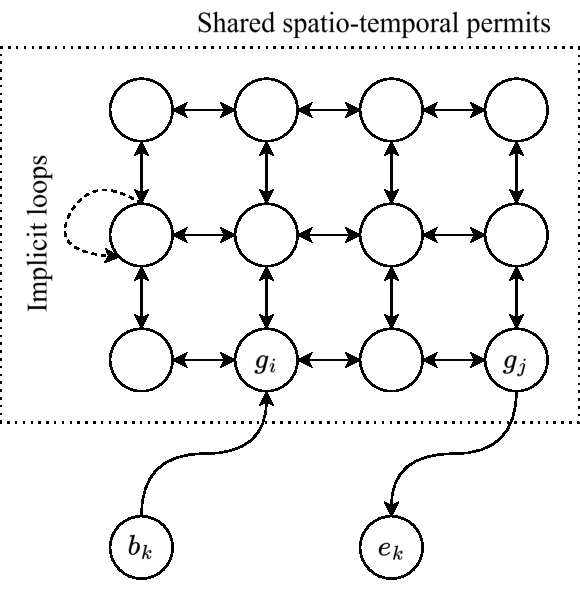
\includegraphics[width=0.8\textwidth]{img/graph_model.pdf}
      \end{columns}
    \end{figure}
\end{frame}


\begin{frame}{MILP Model - Parameters}
    \begin{itemize}
        \item $T$: Maximum time allowed for the mission.
        \item $b_k$: Initial virtual vertex representing the initial position of drone $k$.
        \item $e_k$: Final virtual vertex representing the final position of drone $k$.
        \item $\mathcal{R}$: Set of drones.
        \item $\mathcal{G}$: Digraph $(\mathcal{V}, \mathcal{A})$ representing the airspace.
        \item $\mathcal{V}$: Set of vertices of $\mathcal{G}$.
        \item $\mathcal{B} \subset \mathcal{V}$: Set of initial virtual vertices $b_k$.
        \item $\mathcal{E} \subset \mathcal{V}$: Set of final virtual vertices $e_k$.
        \item $\mathcal{S}$: Set $\mathcal{V} \setminus (\mathcal{B} \cup \mathcal{E})$.
        \item $\mathcal{A}$: Set of arcs $(i,j) \in \mathcal{A}$ of $\mathcal{G}$.
    \end{itemize}
\end{frame}

\begin{frame}{MILP Model - Variables}
    \begin{itemize}
        \item Decision Variables:
        \begin{itemize}
            \item $x_{i,j,t}^k = 1 \iff$ drone $k$ jumps from $i$ to $j$ at time $t$.
        \end{itemize}
        \item Indices:
        \begin{itemize}
            \item $k$: Drone $\implies k \in \mathcal{R}$.
            \item $t$: Time $\implies 1 \leq t \leq T$.
            \item $i, j, l$: Vertices $\implies i, j, l \in \mathcal{V}$.
        \end{itemize}
    \end{itemize}
\end{frame}


\begin{frame}{MILP Model - Objective Function}
    \begin{itemize}
        \item Minimize the total sum of the number of drone movements:
    \end{itemize}
    \[
    \min
    \sum_{k \in \mathcal{R}}
    \sum_{t=1}^T
    \sum_{ \; (i,j) \in \mathcal{A}:\ j \notin (\mathcal{E} \cup \mathcal{B})} x_{i,j,t}^{k}
    \]
    \begin{itemize}
        \item Minimize the total number of drone movements, counting $n-1$ jumps for each drone that performs $n$ jumps.
    \end{itemize}
\end{frame}

\begin{frame}{MILP Model - Constraints}
    \begin{itemize}
        \item Ensure each drone starts its mission:
    \end{itemize}
    \[
    \sum_{t=1}^{T}
    \sum_{j \in \mathcal{S}}
    x_{b_k,j,t}^k = 1, \quad \forall k \in \mathcal{R}
    \]
    \begin{itemize}
        \item Flow conservation:
    \end{itemize}
    \[
    \sum_{j \in \mathcal{V}} x_{i,j,t-1}^{k} =
    \sum_{l \in \mathcal{V}} x_{j,l,t}^{k}, \quad
    \forall j \in \mathcal{V}, \forall k \in \mathcal{R}, \forall t \in \{2, \ldots, T\}
    \]
\end{frame}

\begin{frame}{MILP Model - Constraints (Cont.)}
    \begin{itemize}
        \item Border condition at time $t=0$:
    \end{itemize}
    \[
    x_{i,j,0}^k = \left\{
    \begin{matrix}
        1, & \text{if}\ i=b_k \land j=b_k,\\
        0, & \text{otherwise}.
    \end{matrix}
    \right.
    \quad \forall k \in \mathcal{R}, \forall (i,j) \in A
    \]
    \begin{itemize}
        \item Mutual exclusion of vertex occupation:
    \end{itemize}
    \[
    \sum_{k \in \mathcal{R}}
    \sum_{j \in \mathcal{V}}
    x_{i,j,t}^{k} \leq 1, \quad \forall j \in \mathcal{V}, \forall t \in \{1, \ldots, T\}
    \]
\end{frame}

\begin{frame}{MILP Model - Mission Accomplishment}
    \begin{itemize}
        \item Ensure each drone completes its mission:
    \end{itemize}
    \[
    \sum_{t=1}^{T}
    \sum_{i \in \mathcal{S}}
    x_{i,e_k,t}^k \geq 1, \quad \forall k \in \mathcal{R}
    \]
\end{frame}

\begin{frame}{Heuristic Approach}
        \begin{itemize}
            \item Utilize distance measure as heuristic metric \cite{Weise2023}.
            \item Organize drones in ascending order (prioritized planning) based on start and end points.
            \item Employ iterative Breadth-First Search (BFS) on temporal graph.
            \item Dynamic constraints update of occupied positions (conflict-based search).
            \item Combine heuristic sorting and iterative BFS for efficient path planning and adaptability.
        \end{itemize}
\end{frame}


\begin{frame}{Algorithm Notation}
    \begin{table}
      \centering
      \caption{Notation used in the Algorithm.}
      \label{tab:notation}
      \begin{tabular}{ll}
        \toprule
        Notation & Definition \\
        \midrule
        $\mathcal{V}$ &Set of vertices in the graph $: (i,j,t)$ \\
        $\mathcal{E}$ & Set of edges  \\
        $\mathcal{D}$ & Set of drones \\
        $\mathcal{S}$ & Set of already scheduled vertices \\
        $\mathcal{P}_d \subseteq \mathcal{V} $ & Path of drone $d$ \\
        $\mathcal{G} = (\mathcal{V},\mathcal{E}) $ & Temporal Graph \\
        \bottomrule
      \end{tabular}
    \end{table}
\end{frame}

\begin{frame}{Heuristic Algorithm Steps}
    \begin{enumerate}
        \item \textbf{Drones Sorting}: Ascending sort using Euclidean Distance.
            \begin{equation}
                \mathcal{D}_{\text{sorted}} = \text{sort}(\mathcal{D}, \text{heuristic})
            \end{equation}
        \item \textbf{Path for Each Drone}: Compute path \(P_d\) using BFS on graph \(\mathcal{G}\).
            \begin{equation}
                \forall d \in \mathcal{D}_{\text{sorted}}: \quad \mathcal{P}_d = \text{BFS}(\mathcal{G}, d)
            \end{equation}
        \item \textbf{Constraints Update}: Update set of already scheduled vertices \(\mathcal{S}\).
            \begin{equation}
                \mathcal{S} = \mathcal{S} \cup \bigcup_{d \in \mathcal{D}_{\text{sorted}}} \mathcal{P}_d
            \end{equation}
    \end{enumerate}
\end{frame}

\begin{frame}{Algorithm Visualization}
    \begin{figure}[h]
    \centering
    \begin{tikzpicture}[scale=.8, every node/.style={minimum size=1cm}]

        % Define quadcopter style
        \tikzset{
            quadcopter/.style={
                quadcopter side,
                fill=white,
                draw=gray,
                minimum width=1cm,
                below=of second-scope, 
            },
        }
        
        % Add another drone
        \node (quadcopterGreen) [quadcopter side, fill=white, draw=greenMW, minimum width=1cm, rotate=0] at (5,1) {};

        \node (quadcopterBrown) [quadcopter side, fill=white, draw=brown, minimum width=1cm, rotate=0] at (5,-11.3) {};

        \node (quadcopterOrange) [quadcopter side, fill=white, draw=orange, minimum width=1cm, rotate=0] at (4.4,-14.3) {};

        \node (quadcopterBlue) [quadcopter side, fill=white, draw=blue, minimum width=1cm, rotate=0] at (-5,-8.2) {};
        
        % Último Escopo (t=6)
        \begin{scope}[yshift=-423, every node/.append style={yslant=0.5, xslant=-1}, yslant=0.5, xslant=-1]

            

            \fill[white, fill opacity=0.9] (0,0) rectangle (5,5);
            
            \draw[step=4mm, black] (0,0) grid (5,5);
            \draw[black, thick] (0,0) rectangle (5,5); % Borders
            \fill[orange] (2.05,2.05) rectangle (2.35,2.35); % center pixel
            \node (centerBegint2) at (2.2,2.2) {B}; % place 'B' in the center
            % \fill[greenMW] (1.65,2.05) rectangle (1.95,2.35); % left
            % \fill[greenMW] (2.45,2.05) rectangle (2.75,2.35); % right
            \fill[orange] (2.05,1.95) rectangle (2.35,1.65); % bottom
            \fill[orange,yshift=-11.2] (2.05,1.95) rectangle (2.35,1.65); % bottom
            \fill[orange,yshift=-22.5] (2.05,1.95) rectangle (2.35,1.65); % bottom
            \fill[orange,yshift=-33.5] (2.05,1.95) rectangle (2.35,1.65); % bottom
            
            %\fill[greenMW] (2.05,2.45) rectangle (2.35,2.75); % top
            % 8 -pixel setting
           
            % \fill[greenMW] (2.75,1.95) rectangle (2.45,1.65); % bottom-right
            % \fill[greenMW] (1.65,1.95) rectangle (1.95,1.65); % bottom-left
            
            \node (landedOrange) at (1.5,0.8) {};

            \node(pathdestinyt6) [black, font=\bfseries] at ([yshift=-45.3]centerBegint2) {E};
        \end{scope}



        % Penúltimo Escopo (t=5)
        \begin{scope}[yshift=-340, every node/.append style={yslant=0.5, xslant=-1}, yslant=0.5, xslant=-1]
            \fill[white, fill] (0,0) rectangle (5,5);
            \draw[step=4mm, black] (0,0) grid (5,5);
            \draw[black, thick] (0,0) rectangle (5,5); % Borders
            \fill[orange!55] (2.05,2.05) rectangle (2.35,2.35); % center pixel
            \node (centerBegint3) at (2.2,2.2) {B}; % place 'B' in the center

            \fill[orange!55,xshift=-22.6] (2.45,2.05) rectangle (2.75,2.35); % most left
            

            \node (landedBrown) at (1.5,0.6) {};

            %\fill[blue] (1.65,2.05) rectangle (1.95,2.35); % left
            % left X
            \draw[orange] (1.65,2.05) -- (1.95,2.35);
            \draw[orange] (1.65,2.35) -- (1.95,2.05);
            % left bottom X
            \draw[orange, yshift=-11.3] (1.65,2.05) -- (1.95,2.35);
            \draw[orange, yshift=-11.3] (1.65,2.35) -- (1.95,2.05);   
            % most left X
            \draw[orange, xshift=-11.3] (1.65,2.05) -- (1.95,2.35);
            \draw[orange, xshift= -11.3] (1.65,2.35) -- (1.95,2.05);   

            \fill[orange!55,xshift=11.3] (2.45,2.05) rectangle (2.75,2.35); % most right
            % most right X
            \draw[orange, xshift=34.4] (1.65,2.05) -- (1.95,2.35);
            \draw[orange, xshift=34.4] (1.65,2.35) -- (1.95,2.05);

            % bottom center right X
            \draw[orange, xshift=34.4, yshift= -11.3] (1.65,2.05) -- (1.95,2.35);
            \draw[orange, xshift=34.4, yshift= -11.3] (1.65,2.35) -- (1.95,2.05);

            %  top center right X
            \draw[orange, xshift=34.4, yshift= 11.3] (1.65,2.05) -- (1.95,2.35);
            \draw[orange, xshift=34.4, yshift= 11.3] (1.65,2.35) -- (1.95,2.05);
            
            % most most right X
            \draw[orange, xshift=34.4 + 11.3] (1.65,2.05) -- (1.95,2.35);
            \draw[orange, xshift=34.4 + 11.3] (1.65,2.35) -- (1.95,2.05);

            

            \fill[orange!55] (2.45,2.05) rectangle (2.75,2.35); % right
            
            \fill[orange!55] (2.05,2.45) rectangle (2.35,2.75); % top
            \fill[orange!55, xshift=11.3] (2.05,2.45) rectangle (2.35,2.75); % top right
            \fill[orange!55, xshift=-11.3] (2.05,2.45) rectangle (2.35,2.75); % top left
            \fill[orange!55, yshift=11.3] (2.05,2.45) rectangle (2.35,2.75); % most top
            \fill[orange!55] (2.05,1.95) rectangle (2.35,1.65); % bottom

            \fill[orange!55, xshift= 11.3] (2.05,1.95) rectangle (2.35,1.65); % bottom right

            \fill[orange!55,yshift=-11.3] (2.05,1.95) rectangle (2.35,1.65); % most bottom
            
            %\fill[greenMW] (1.65,2.45) rectangle (1.95,2.75); % top-left 
            % top left X
            \draw[orange] (1.65,2.75) -- (1.95,2.45);
            \draw[orange] (1.65,2.45) -- (1.95,2.75);
            
            % top most left X
            \draw[orange, xshift=-11.3] (1.65,2.75) -- (1.95,2.45);
            \draw[orange, xshift=-11.3] (1.65,2.45) -- (1.95,2.75);
            
            % \draw[orange,xshift=-11.3] (1.65,2.75) -- (1.95,2.45);
            % \draw[orange,xshift=-11.3] (1.65,2.45) -- (1.95,2.75);   

            %\fill[greenMW] (2.45,2.45) rectangle (2.75,2.75); % top-right
            \draw[orange] (2.45,2.45) -- (2.75,2.75);
            \draw[orange] (2.45,2.75) -- (2.75,2.45);

            %\fill[greenMW] (2.75,1.95) rectangle (2.45,1.65); % bottom-right
            \draw[orange] (2.45,1.95) -- (2.75,1.65);
            \draw[orange] (2.45,1.65) -- (2.75,1.95);

            % top most X 
            \draw[orange,xshift= -34 +45.4,yshift=11] (1.65,2.75) -- (1.95,2.45);
            \draw[orange,xshift=-34 +45.4,yshift=11] (1.65,2.45) -- (1.95,2.75);

            % top most right X 
            \draw[orange,xshift= -34 +45.4 + 11.2,yshift=11] (1.65,2.75) -- (1.95,2.45);
            \draw[orange,xshift=-34 +45.4 + 11.2,yshift=11] (1.65,2.45) -- (1.95,2.75);

            % top most left X 
            \draw[orange,xshift= -34 +45.4 - 11.2,yshift=11] (1.65,2.75) -- (1.95,2.45);
            \draw[orange,xshift=-34 +45.4 - 11.2,yshift=11] (1.65,2.45) -- (1.95,2.75);

            % top most last X 
            \draw[orange,xshift= -34 +45.4 ,yshift=22.2] (1.65,2.75) -- (1.95,2.45);
            \draw[orange,xshift=-34 +45.4 ,yshift=22.2] (1.65,2.45) -- (1.95,2.75);

            % bottom most X
            \draw[orange,xshift= -34 +45.4,yshift=-34.4] (1.65,2.75) -- (1.95,2.45);
            \draw[orange,xshift=-34 +45.4,yshift=-34.4] (1.65,2.45) -- (1.95,2.75);

            % bottom most right X
            \draw[orange,xshift= -34 +45.4 +11.2 ,yshift=-34.4] (1.65,2.75) -- (1.95,2.45);
            \draw[orange,xshift=-34 +45.4 + 11.2,yshift=-34.4] (1.65,2.45) -- (1.95,2.75);

            % bottom most left X
            \draw[orange,xshift= -34 +45.4 -11.2 ,yshift=-34.4] (1.65,2.75) -- (1.95,2.45);
            \draw[orange,xshift=-34 +45.4  -11.2,yshift=-34.4] (1.65,2.45) -- (1.95,2.75);

            % bottom most last X
            \draw[orange,xshift= -34 +45.4,yshift=-45.8] (1.65,2.75) -- (1.95,2.45);
            \draw[orange,xshift=-34 +45.4,yshift=-45.8] (1.65,2.45) -- (1.95,2.75);

                    

            %\fill[blue] (1.65,1.95) rectangle (1.95,1.65); % bottom-left
            % 2. ring
            %\fill[greenMW] (1.25,1.55) rectangle (1.55,1.25); % bottom-left
            %\fill[greenMW] (0.85,1.55) rectangle (1.15,1.25); % bottom-left
            %\fill[greenMW] (0.85,1.15) rectangle (1.15,0.85); % bottom-left

            \fill[brown, xshift=22.7, yshift=-11.2] (1.25,0.75) rectangle (1.55,0.45); % bottom-left

            \node(pathdestinyt3) [black, font=\bfseries] at ([yshift=-45.3]centerBegint3) {E};
        \end{scope}


        % Escopo (t=4)
        \begin{scope}[yshift=-250, every node/.append style={yslant=0.5, xslant=-1}, yslant=0.5, xslant=-1]
            \fill[white, fill] (0,0) rectangle (5,5);
            \draw[step=4mm, black] (0,0) grid (5,5);
            \draw[black, thick] (0,0) rectangle (5,5); % Borders
            \fill[orange!55] (2.05,2.05) rectangle (2.35,2.35); % center pixel
            \node (centerBegint3) at (2.2,2.2) {B}; % place 'B' in the center
            
            %\fill[blue] (1.65,2.05) rectangle (1.95,2.35); % left
            \draw[orange] (1.65,2.05) -- (1.95,2.35);
            \draw[orange] (1.65,2.35) -- (1.95,2.05);   

            \node (landedBlue) at (1.1,2.3) {};

            % most right X
            \draw[orange, xshift=34.4] (1.65,2.05) -- (1.95,2.35);
            \draw[orange, xshift=34.4] (1.65,2.35) -- (1.95,2.05);  

            \fill[orange!55] (2.45,2.05) rectangle (2.75,2.35); % right
            \fill[orange!55] (2.05,2.45) rectangle (2.35,2.75); % top
            \fill[orange!55] (2.05,1.95) rectangle (2.35,1.65); % bottom
            
            %\fill[greenMW] (1.65,2.45) rectangle (1.95,2.75); % top-left
            \draw[orange] (1.65,2.75) -- (1.95,2.45);
            \draw[orange] (1.65,2.45) -- (1.95,2.75);   
            
            % \draw[orange,xshift=-11.3] (1.65,2.75) -- (1.95,2.45);
            % \draw[orange,xshift=-11.3] (1.65,2.45) -- (1.95,2.75);   

            %\fill[greenMW] (2.45,2.45) rectangle (2.75,2.75); % top-right
            \draw[orange] (2.45,2.45) -- (2.75,2.75);
            \draw[orange] (2.45,2.75) -- (2.75,2.45);

            %\fill[greenMW] (2.75,1.95) rectangle (2.45,1.65); % bottom-right
            \draw[orange] (2.45,1.95) -- (2.75,1.65);
            \draw[orange] (2.45,1.65) -- (2.75,1.95);

            % top most X 
            \draw[orange,xshift= -34 +45.4,yshift=11] (1.65,2.75) -- (1.95,2.45);
            \draw[orange,xshift=-34 +45.4,yshift=11] (1.65,2.45) -- (1.95,2.75);

            % bottom most X
            \draw[orange,xshift= -34 +45.4,yshift=-34.4] (1.65,2.75) -- (1.95,2.45);
            \draw[orange,xshift=-34 +45.4,yshift=-34.4] (1.65,2.45) -- (1.95,2.75);

            \fill[blue] (1.65,1.95) rectangle (1.95,1.65); % bottom-left
            % 2. ring
            %\fill[greenMW] (1.25,1.55) rectangle (1.55,1.25); % bottom-left
            %\fill[greenMW] (0.85,1.55) rectangle (1.15,1.25); % bottom-left
            %\fill[greenMW] (0.85,1.15) rectangle (1.15,0.85); % bottom-left

            \fill[brown, xshift=22.6] (1.25,0.75) rectangle (1.55,0.45); % bottom-left

            \node(pathdestinyt3) [black, font=\bfseries] at ([yshift=-45.3]centerBegint3) {E};
        \end{scope}

        % Terceiro Escopo (t=3)
        \begin{scope}[yshift=-166, every node/.append style={yslant=0.5, xslant=-1}, yslant=0.5, xslant=-1]
            \fill[white, fill opacity=0.9] (0,0) rectangle (5,5);
            \draw[step=4mm, black] (0,0) grid (5,5);
            \draw[black, thick] (0,0) rectangle (5,5); % Borders
            \fill[orange!55] (2.05,2.05) rectangle (2.35,2.35); % lighter orange for center pixel
            \node (centerBegint3) at (2.2,2.2) {B}; % place 'B' in the center
            \fill[blue] (1.65,2.05) rectangle (1.95,2.35); % left
            \draw[orange] (2.45,2.05) -- (2.75,2.35);
            \draw[orange] (2.45,2.35) -- (2.75,2.05);
            %\fill[greenMW] (2.05,2.45) rectangle (2.35,2.75); % top
            \draw[orange] (2.05,2.45) -- (2.35,2.75);
            \draw[orange] (2.05,2.75) -- (2.35,2.45);

            %\fill[greenMW] (2.05,1.95) rectangle (2.35,1.65); % bottom
            \draw[orange] (2.05,1.95) -- (2.35,1.65);
            \draw[orange] (2.05,1.65) -- (2.35,1.95);

            
            %\fill[greenMW] (1.65,2.45) rectangle (1.95,2.75); % top-left
            %\fill[greenMW] (2.45,2.45) rectangle (2.75,2.75); % top-right
            %\fill[greenMW] (2.75,1.95) rectangle (2.45,1.65); % bottom-right
            %\fill[greenMW] (1.65,1.95) rectangle (1.95,1.65); % bottom-left
            % 2. ring
            %\fill[greenMW] (1.25,1.55) rectangle (1.55,1.25); % bottom-left
            %\fill[greenMW] (0.85,1.55) rectangle (1.15,1.25); % bottom-left
            %\fill[greenMW] (0.85,1.15) rectangle (1.15,0.85); % bottom-left

            \fill[brown, xshift=11.3] (1.25,0.75) rectangle (1.55,0.45); % bottom-left

            \node(pathdestinyt3) [black, font=\bfseries] at ([yshift=-45.3]centerBegint3) {E};

            \node(midpointX) at (2.6, 2.2){};
            
        \end{scope}

        % Escopo do meio (t=2)
        \begin{scope}[yshift=-83, every node/.append style={yslant=0.5, xslant=-1}, yslant=0.5, xslant=-1]

            \node [quadcopter side,fill=white,draw=orange,minimum width=1cm,rotate=10] (quadcoptert2) at (1,7) {};

            \fill[white, fill opacity=0.9] (0,0) rectangle (5,5);

            \node (arrivalOrange) at (1.8,2.1) {};
            
            \draw[step=4mm, black] (0,0) grid (5,5);
            \draw[black, thick] (0,0) rectangle (5,5); % Borders
            \fill[orange] (2.05,2.05) rectangle (2.35,2.35); % center pixel
            \node (centerBegint2) at (2.2,2.2) {B}; % place 'B' in the center
            % \fill[greenMW] (1.65,2.05) rectangle (1.95,2.35); % left
            % \fill[greenMW] (2.45,2.05) rectangle (2.75,2.35); % right
            \fill[greenMW] (2.05,1.95) rectangle (2.35,1.65); % bottom
            \node (landedGreen) at (1.8,1.9) {};
            %\fill[greenMW] (2.05,2.45) rectangle (2.35,2.75); % top
            % 8 -pixel setting
            \fill[blue] (1.65,2.45) rectangle (1.95,2.75); % top-left
            % \fill[greenMW] (2.45,2.45) rectangle (2.75,2.75); % top-right
            % \fill[greenMW] (2.75,1.95) rectangle (2.45,1.65); % bottom-right
            % \fill[greenMW] (1.65,1.95) rectangle (1.95,1.65); % bottom-left
            % 2. ring
            % \fill[greenMW] (1.25,1.55) rectangle (1.55,1.25); % bottom-left
            % \fill[greenMW] (0.85,1.55) rectangle (1.15,1.25); % bottom-left
            % \fill[greenMW] (0.85,1.15) rectangle (1.15,0.85); % bottom-left
            \fill[brown] (1.25,0.75) rectangle (1.55,0.45); % bottom-left
            \node(pathdestinyt2) [black, font=\bfseries] at ([yshift=-45.3]centerBegint2) {E};
        \end{scope}

        % Primeiro Escopo (t=1)
        \begin{scope}[yshift=0, every node/.append style={yslant=0.5, xslant=-1}, yslant=0.5, xslant=-1]

           \node [quadcopter side,fill=white,draw=orange,minimum width=1cm,rotate=10] (quadcoptert1) at (3,7.6) {};
            
           \node (orangeTakeOff) at (2.5,1.8) {};
        
            \fill[white, fill opacity=0.9] (0,0) rectangle (5,5);
            \draw[step=4mm, black] (0,0) grid (5,5); % Grid definition
            \draw[black, thick] (0,0) rectangle (5,5); % Borders
            \fill[greenMW] (2.05,2.05) rectangle (2.35,2.35); % center pixel
            \draw[red, thin] (2.05,2.05) rectangle (2.35,2.35); % border
            \node (centerBegint1) at (2.2,2.2) {B}; % place 'B' in the center
            \fill[blue] (2.05,2.45) rectangle (2.35,2.75); % top
            % \fill[blue] (1.65,2.45) rectangle (1.95,2.75); % top-left
            % \fill[blue] (2.45,2.45) rectangle (2.75,2.75); % top-right
            % \fill[blue] (2.75,1.95) rectangle (2.45,1.65); % bottom-right
            % \fill[blue] (1.65,1.95) rectangle (1.95,1.65); % bottom-left
            % % 2. ring
            % \fill[blue] (1.25,1.55) rectangle (1.55,1.25); % bottom-left
            % \fill[blue] (0.85,1.55) rectangle (1.15,1.25); % bottom-left
            % \fill[blue] (0.85,1.15) rectangle (1.15,0.85); % bottom-left
            % \fill[blue] (1.25,0.75) rectangle (1.55,0.45); % bottom-left

            \fill[brown, xshift= -11.3] (1.25,0.75) rectangle (1.55,0.45); % bottom-left
            
            % Insert 'E' three squares down the center
            \node(pathdestinyt1) [black, font=\bfseries] at ([yshift=-45.3]centerBegint1) {E};
            
        \end{scope}

        % Draw annotations
        \draw[-latex, thick, gray, dashed] (-5.4,-3.5) node[left] {occupied} to[out=0, in=200] (-0.5,-4.1);

        \draw[-latex, thick, red] (quadcoptert1) to[out=35, in=90] node[midway, above] {failed takeoff} (orangeTakeOff);

        \draw[-latex, thick, orange] (quadcoptert2) to[out=0, in=10] node[very near start, above] {arrival} (arrivalOrange);

        %\draw[-latex, thick, orange] ([xshift=-10]centerBegint3) to[out=0, in=10] (midpointX);

        \draw[thick, green!60!black, dashed] (landedGreen) to[out=0, in=10] node[above, pos=0.45 , font=\footnotesize] {landed} (quadcopterGreen);

        \draw[thick, brown!, dashed] (landedBrown) to[out=0, in=10] node[ above, pos=1 , font=\footnotesize] {landed} (quadcopterBrown);

        \draw[thick, orange!, dashed] (landedOrange) to[out=0, in=10] node[ above, pos=0.75 , font=\footnotesize] {path found} (quadcopterOrange);

        \draw[thick, blue!60!white, dashed] (landedBlue) to[out=0, in=13] node[ above, pos=0.85 , font=\footnotesize] {landed} (quadcopterBlue);

        % Annotations
        \draw[thick, gray!60!black] (6,4) node {t=1};
        \draw[thick, gray!60!black] (6,0) node {t=2};
        \draw[thick, gray!60!black] (6,-3) node {t=3};
        \draw[thick, gray!60!black] (6,-6) node {t=4};
        \draw[thick, gray!60!black] (6,-9) node {t=5};
        \draw[thick, gray!60!black] (6.2,-12.4) node {t=6};
    \end{tikzpicture}
    \caption{Algorithm visualization. Source: The authors.}
    \label{fig:visualgo}
\end{figure}

\end{frame}

\begin{frame}{Complexity Analysis and Boundedness}
    \begin{itemize}
        \item Worst-case complexity: $\mathcal{O}((N+M) K N M \log((N+M) K N M))$.
        \item Approximation: $\mathcal{O}(N^3 K \log(N^3 K))$ for square grids.
    \end{itemize}
    \begin{figure}
      \centering
      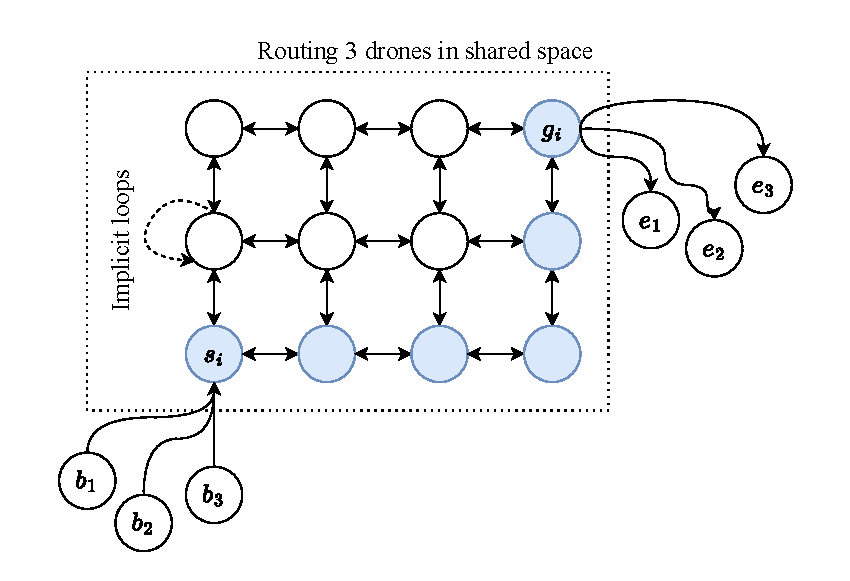
\includegraphics[width=0.6\textwidth]{img/worst_path.drawio.pdf}
      \caption{Worst case path. Source: The authors.}
      \label{fig:worst_path}
    \end{figure}
\end{frame}

\begin{frame}{Hybrid Methodology}
    \begin{itemize}
        \item \textbf{Heuristic Solution Generation}
            \begin{itemize}
                \item Quickly generates an initial feasible solution.
                \item Determines a plausible time horizon $T_{\text{heuristic}}$.
            \end{itemize}
        \item \textbf{MILP Model Refinement}
            \begin{itemize}
                \item Uses $T_{\text{heuristic}}$ and initial feasible solution from heuristic.
                \item Refines the solution to ensure global optimality.
            \end{itemize}
        \item \textbf{Advantages}
            \begin{itemize}
                \item Combines computational speed with solution accuracy.
                \item Skips multiple iterations to determine $T$, reducing computational expense.
            \end{itemize}
    \end{itemize}
\end{frame}

